\chapter{Analisi proporzionale di Coben}

Quest'analisi\footcite{Coben1979,Manetti1984,Coben1985,Antonini1986} inquadra il cranio in un sistema di coordinate rettangolare, in cui l'asse orizzontale delle ascisse è il \textit{Basion Orizzontale} (\punto{BaH}), il punto d'origine è il \textit{Basion} (\punto{Ba}), e l'asse delle ordinate è il \textit{Basion Verticale} (\punto{BaV}). L'asse delle ascisse, in questo sistema, è parallelo al \emph{piano di Francoforte} \punto{FH}. Le misurazioni della profondità facciale sono l'espressione della componente orizzontale della crescita, relativa al \textit{forame occipitale} (o \textit{forame magno}). In maniera simile, le misurazioni dell'altezza facciale sono espressione della componente verticale di crescita, relativa al forame occipitale.

Le misurazioni orizzontali vengono prese parallelamente a \punto{BaH}, quelle verticali parallelamente a \punto{BaV}. Il sistema di coordinate rettangolare permette misure lineari dei segmenti craniofacciali e, attraverso un sistema di proporzioni, la valutazione dei rapporti tra i singoli segmenti, fornendo un profilo individuale.

Quest'analisi quantifica ed esprime la crescita cefalometrica analizzando cinque regioni: base cranica, profondità facciale, altezza facciale, elementi dentari e profilo.

%si compone di tre parti: l'indice di profondità, la profondità e l'equilibrio verticale. Non vengono utilizzati punti cefalometrici particolari, a parte \textit{Incision superiore (Is)} e \textit{Incision inferiore (Ii)}, già descritti nell'analisi di Ricketts.

%\section{Descrizione}
% \subsection{Valutazione dell'indice di profondità}
% È possibile definire \textit{indice di profondità} il rapporto tra l'altezza facciale anteriore (\piano{Na}{Me}) e la profondità facciale (\piano{Ba}{Na}). I valori medio-normali di questo rapporto, utile nel fornire indicazioni sull'armonia dello sviluppo facciale, sono di $115,5 \pm 6,56$ in fase di dentatura mista e $123,9 \pm 4,85$ in dentatura permanente.

\section{Analisi della profondità}
% Per descrivere l'analisi della profondità facciale, è utile suddividerla in tre livelli:
% \begin{itemize}
% \item livello ``base cranica''
% \item livello ``mascellare superiore''
% \item livello ``mandibola''
% \end{itemize}

\subsection*{Base cranica}
\begin{figure}
\centering
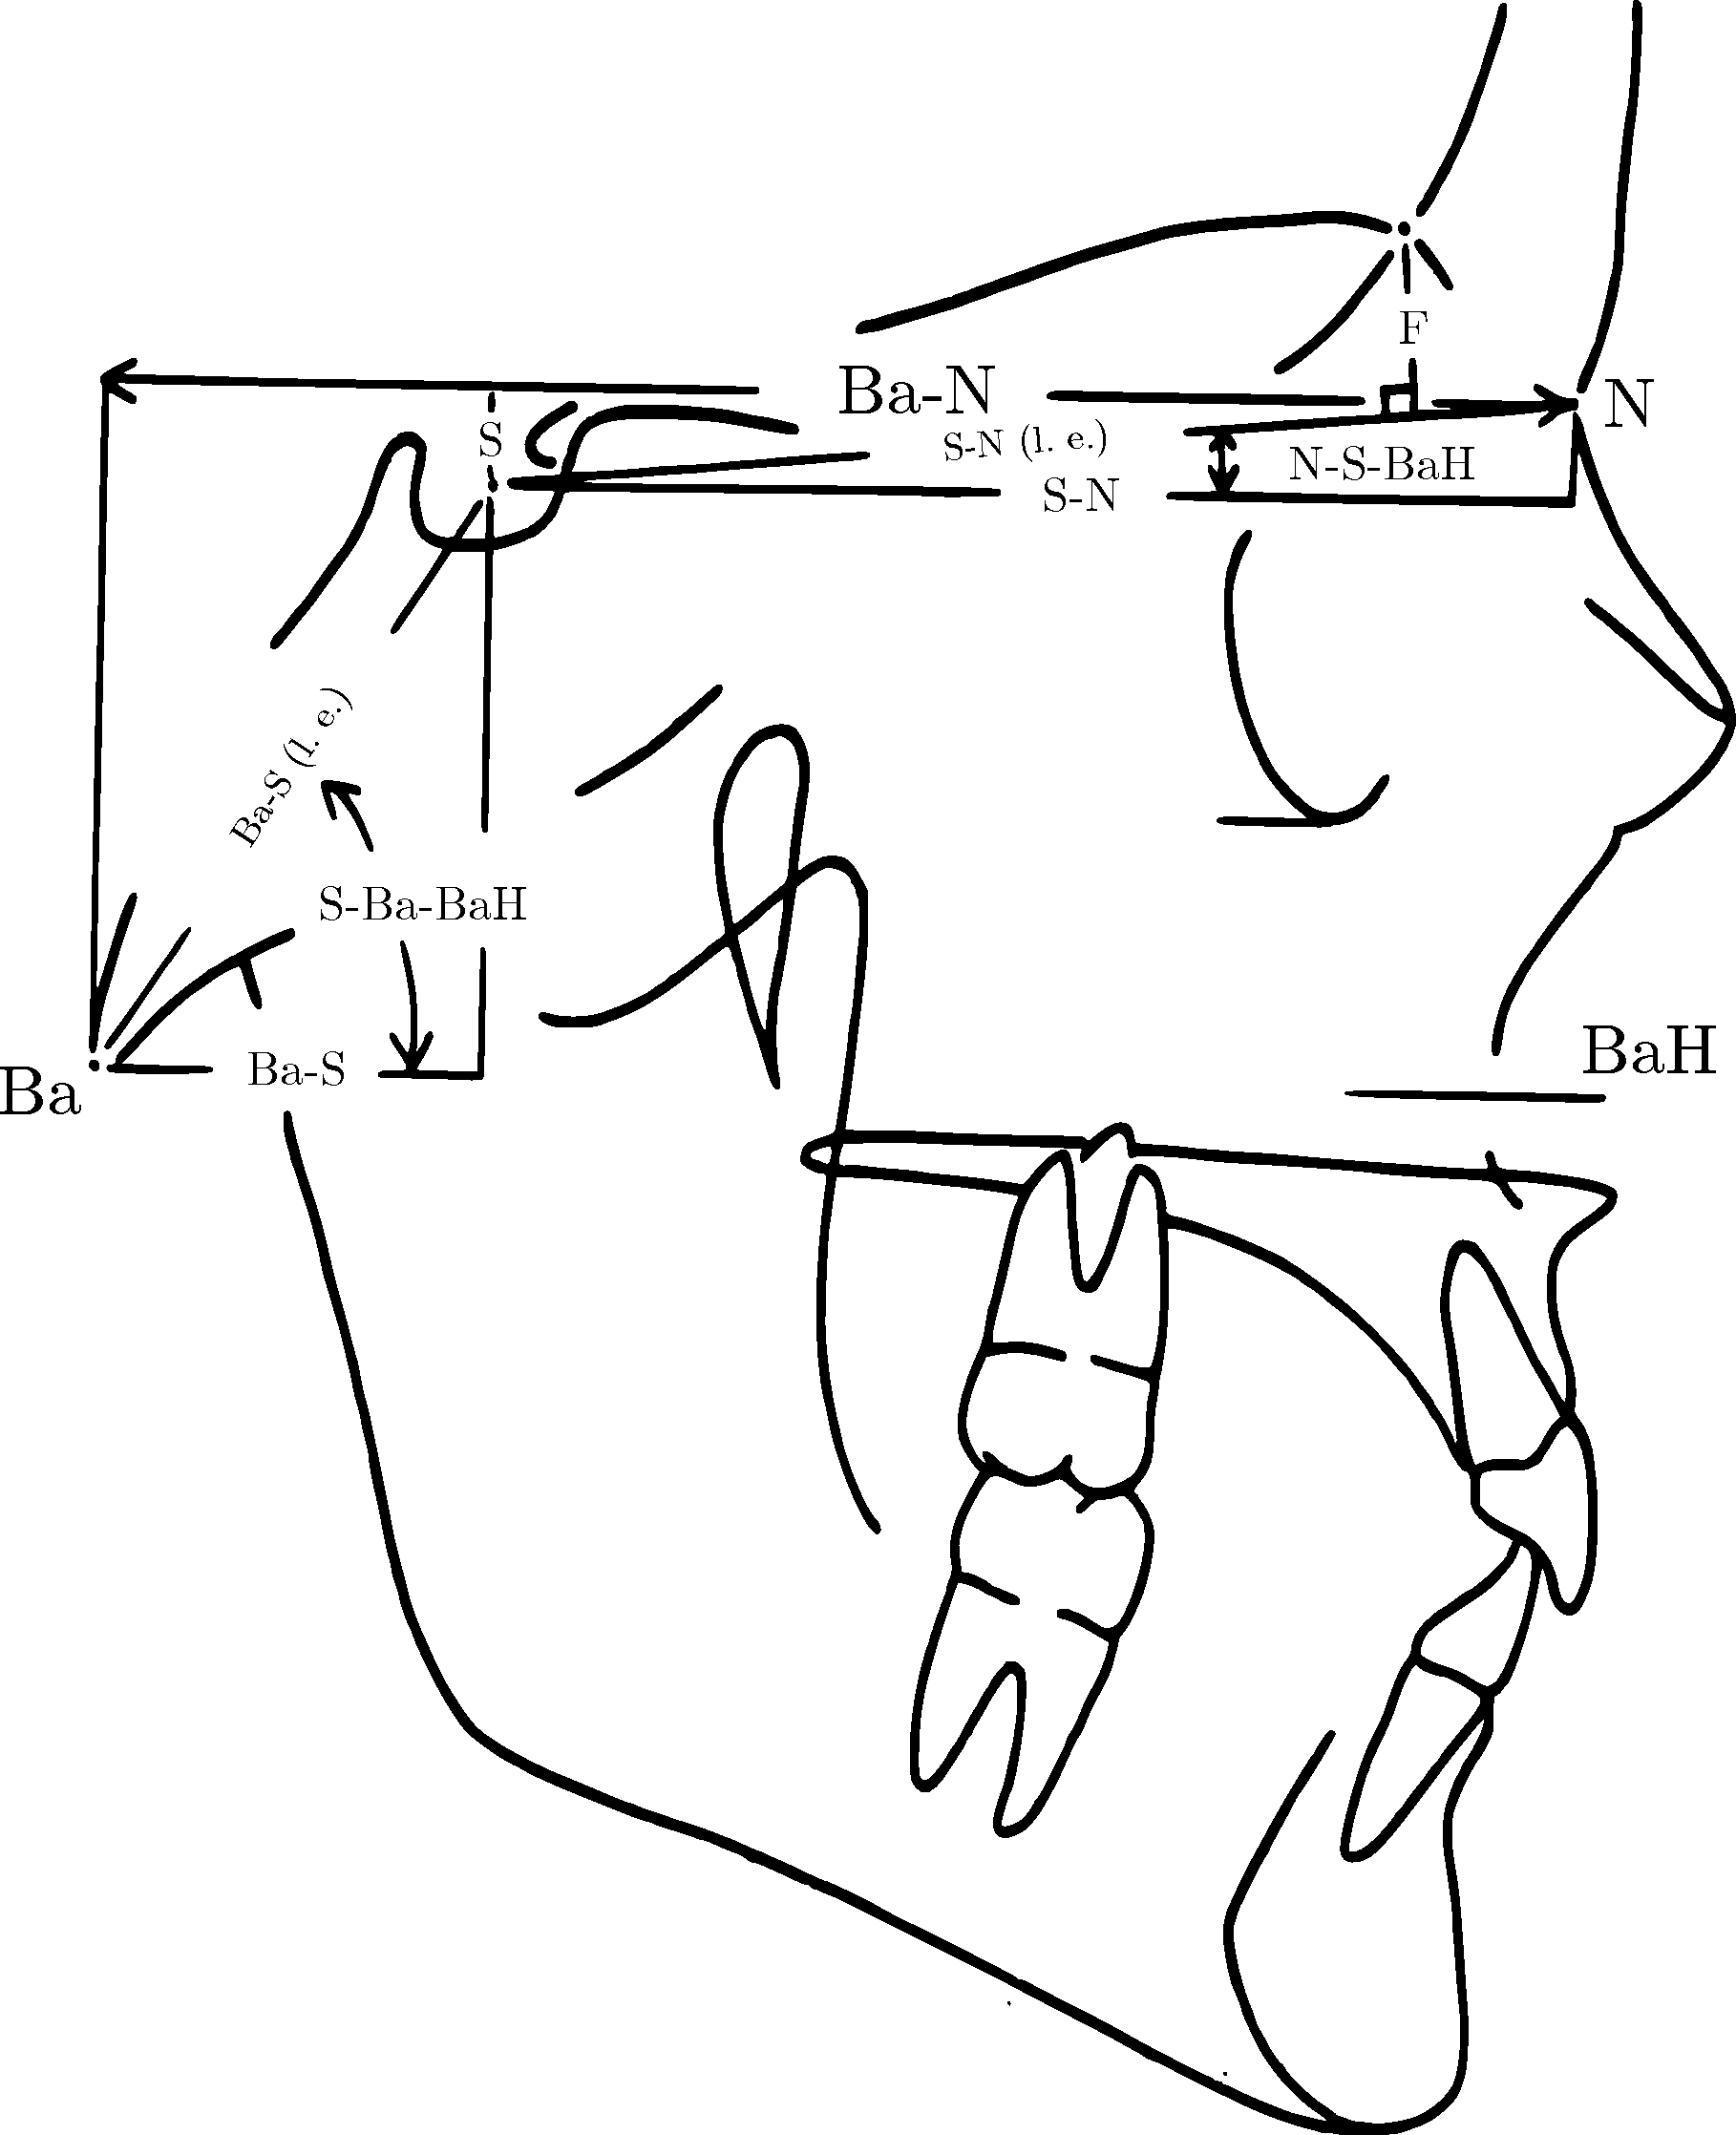
\includegraphics[width=.6\columnwidth]{./images/coben_base_cranica.pdf}
\caption{Analisi della base cranica secondo Coben}
\label{fig:coben_base_cranica}
\end{figure}

\paragraph{Profondità totale effettiva della base cranica} \piano{Ba}{N}, è una delle poche misure assolute di quest'analisi. È propria di ciascun soggetto, e ad essa vengono rapportate tutte le misure antero-posteriori. Il suo valore medio è di $83,1 \pm 3,75$mm. Essa viene suddivisa in \textbf{profondità della base cranica posteriore} e \textbf{profondità della base cranica anteriore}.

\paragraph{Profondità della base cranica posteriore} \piano{Ba}{S}, rappresenta il contributo della parte posteriore alla profondità totale della base cranica. Essa varia al variare della lunghezza del tratto \piano{Ba}{S} e della sua inclinazione rispetto al \punto{BaH}. Più questo piano è orizzontale, più la sua dimensione e la sua crescita contribuisce alla profondità craniofacciale; più è verticale, più contribuisce all'altezza. È questa misura che riflette l'entità e la direzione di crescita della sincondrosi sfeno-occipitale.

\paragraph{Profondità della base cranica anteriore} \piano{S}{N}, è simile all'analogo posteriore: anch'esso viene misurato in termini angolari in relazione al \punto{BaH}. Poiché il processo di crescita della base cranica anteriore si modifica dopo i sette anni, la porzione \piano{S}{N} viene suddivisa in un segmento che può essere considerato rappresentativo della vera base cranica, e in un segmento che rappresenta lo spessore dell'osso frontale. Anatomicamente, i limiti della base cranica anteriore sarebbe rappresentanto dal tratto tra la fossa dell'ipofisi al forame cieco. Poiché quest'ultimo non è radiograficamente visibile, viene utilizzato un punto cefalometrico, il \emph{frontale}, definito come il punto di mezzo tra le immagini del soffitto delle orbite, nel punto in cui incrociano la lamina interna dell'osso frontale. Questo punto di repere viene quindi proiettato su \piano{S}{N} in maniera perpendicolare: questo sarà il \emph{frontale costruito} \punto{F}. I due segmenti in cui viene diviso \piano{S}{N} sono quindi \piano{S}{F} e \piano{F}{N}. Fino a circa 7 anni, la crescita di \piano{S}{N} si esplica tutta nel tratto \piano{S}{F}, con la crescita della sutura sfeno-etmoidale. Con la chiusura di questa, il segmento \piano{S}{F} si stabilizza, mentre il tratto \piano{F}{N} mostra un aumento (dovuto all'ispessimento dell'osso frontale). Misurando l'angolo della base cranica posteriore (\punto{S}-\punto{Ba}-\punto{BaH}, indicato con \punto{BaS}$\measuredangle$), e l'angolo della base cranica anteriore (\punto{N}-\punto{S}-\punto{BaH}, indicato con \punto{SN}$\measuredangle$), si sta effettivamente misurando l'effetto combinato dell'angolo della base cranica, e della postura della testa, sulle effettive profondità ed altezza della base cranica totale, \piano{Ba}{N}. Queste variabili sono correlate tra loro secondo l'equazione:
\begin{equation}
S\measuredangle = 180° + (SN\measuredangle) - BaS\measuredangle
\end{equation}

%\paragraph{Profondità del basisfenoide} \piano{Ba}{S}/\piano{Ba}{Na} o, in altri termini, l'inclinazione della fossa cranica media. Il suo valore medio è di $25,4 \pm 1,4$\%.

\subsection*{Profondità facciale}
\begin{table}[h]
\centering
\caption{Valori medi della profondità facciale nell'analisi di Coben}
\label{tab:coben_profondita_facciale}
\begin{tabular}{lcD{,}{,}{3.3}D{,}{,}{3.3}}
\toprule
\multicolumn{1}{c}{\textbf{Segmento}} & \multicolumn{1}{c}{\textbf{Riferimento}} & \multicolumn{1}{c}{\textbf{Valore medio}} & \multicolumn{1}{c}{\textbf{Dev. Std.}} \\
\midrule
\piano{Ba}{S} & \piano{Ba}{N} & 24,9 \% & 2,16 \\
\piano{S}{Ptm} & & 20,7 \% & 2,47 \\
\piano{Ptm}{A} & & 51,4 \% & 2,59 \\
\piano{Ba}{A} & & 97,0 \% & 3,24 \\
\piano{Ba}{Ar} & & 9,9 \% & 2,60 \\
\piano{Ar}{Pog} & & 80,2 \% & 6,48 \\
\piano{Ba}{B} & & 90,1 \% & 5,50 \\
\piano{Ba}{Pog} & & 90,1 \% & 6,38 \\
\piano{Ar}{Go} & & 7,6 \% & 3,95 \\
\piano{B}{Pog} & & 0,0 \% & 1,78 \\
\piano{Go}{Pog} & & 72,6 \% & 4,44 \\
\bottomrule
\end{tabular}
\end{table}

\paragraph{Profondità media facciale} viene misurata parallela a \punto{BaH} dal punto \punto{Ba} al punto \punto{A}. Tale profondità può essere suddivisa in tre tratti: il contributo della base cranica posteriore \piano{Ba}{S}, il contributo delle lamine pterigoidee, misurato come \piano{S}{Ptm} (media $20,7 \pm 2,47\%$ di \piano{Ba}{N}) e la profondità del mascellare superiore \piano{Ptm}{A} (media $51,4 \pm 2,59\%$ di \piano{Ba}{N}). La misura lineare di ognuno di questi segmenti viene sommata a formare la profondità media facciale totale. Per valutare se questa misura è in equilibrio con le altre strutture, è necessario rapportarla alla profondità totale della base cranica: la media è di $97,0 \pm 3,24\%$ di \piano{Ba}{N}.

\begin{figure}[ht]
\centering
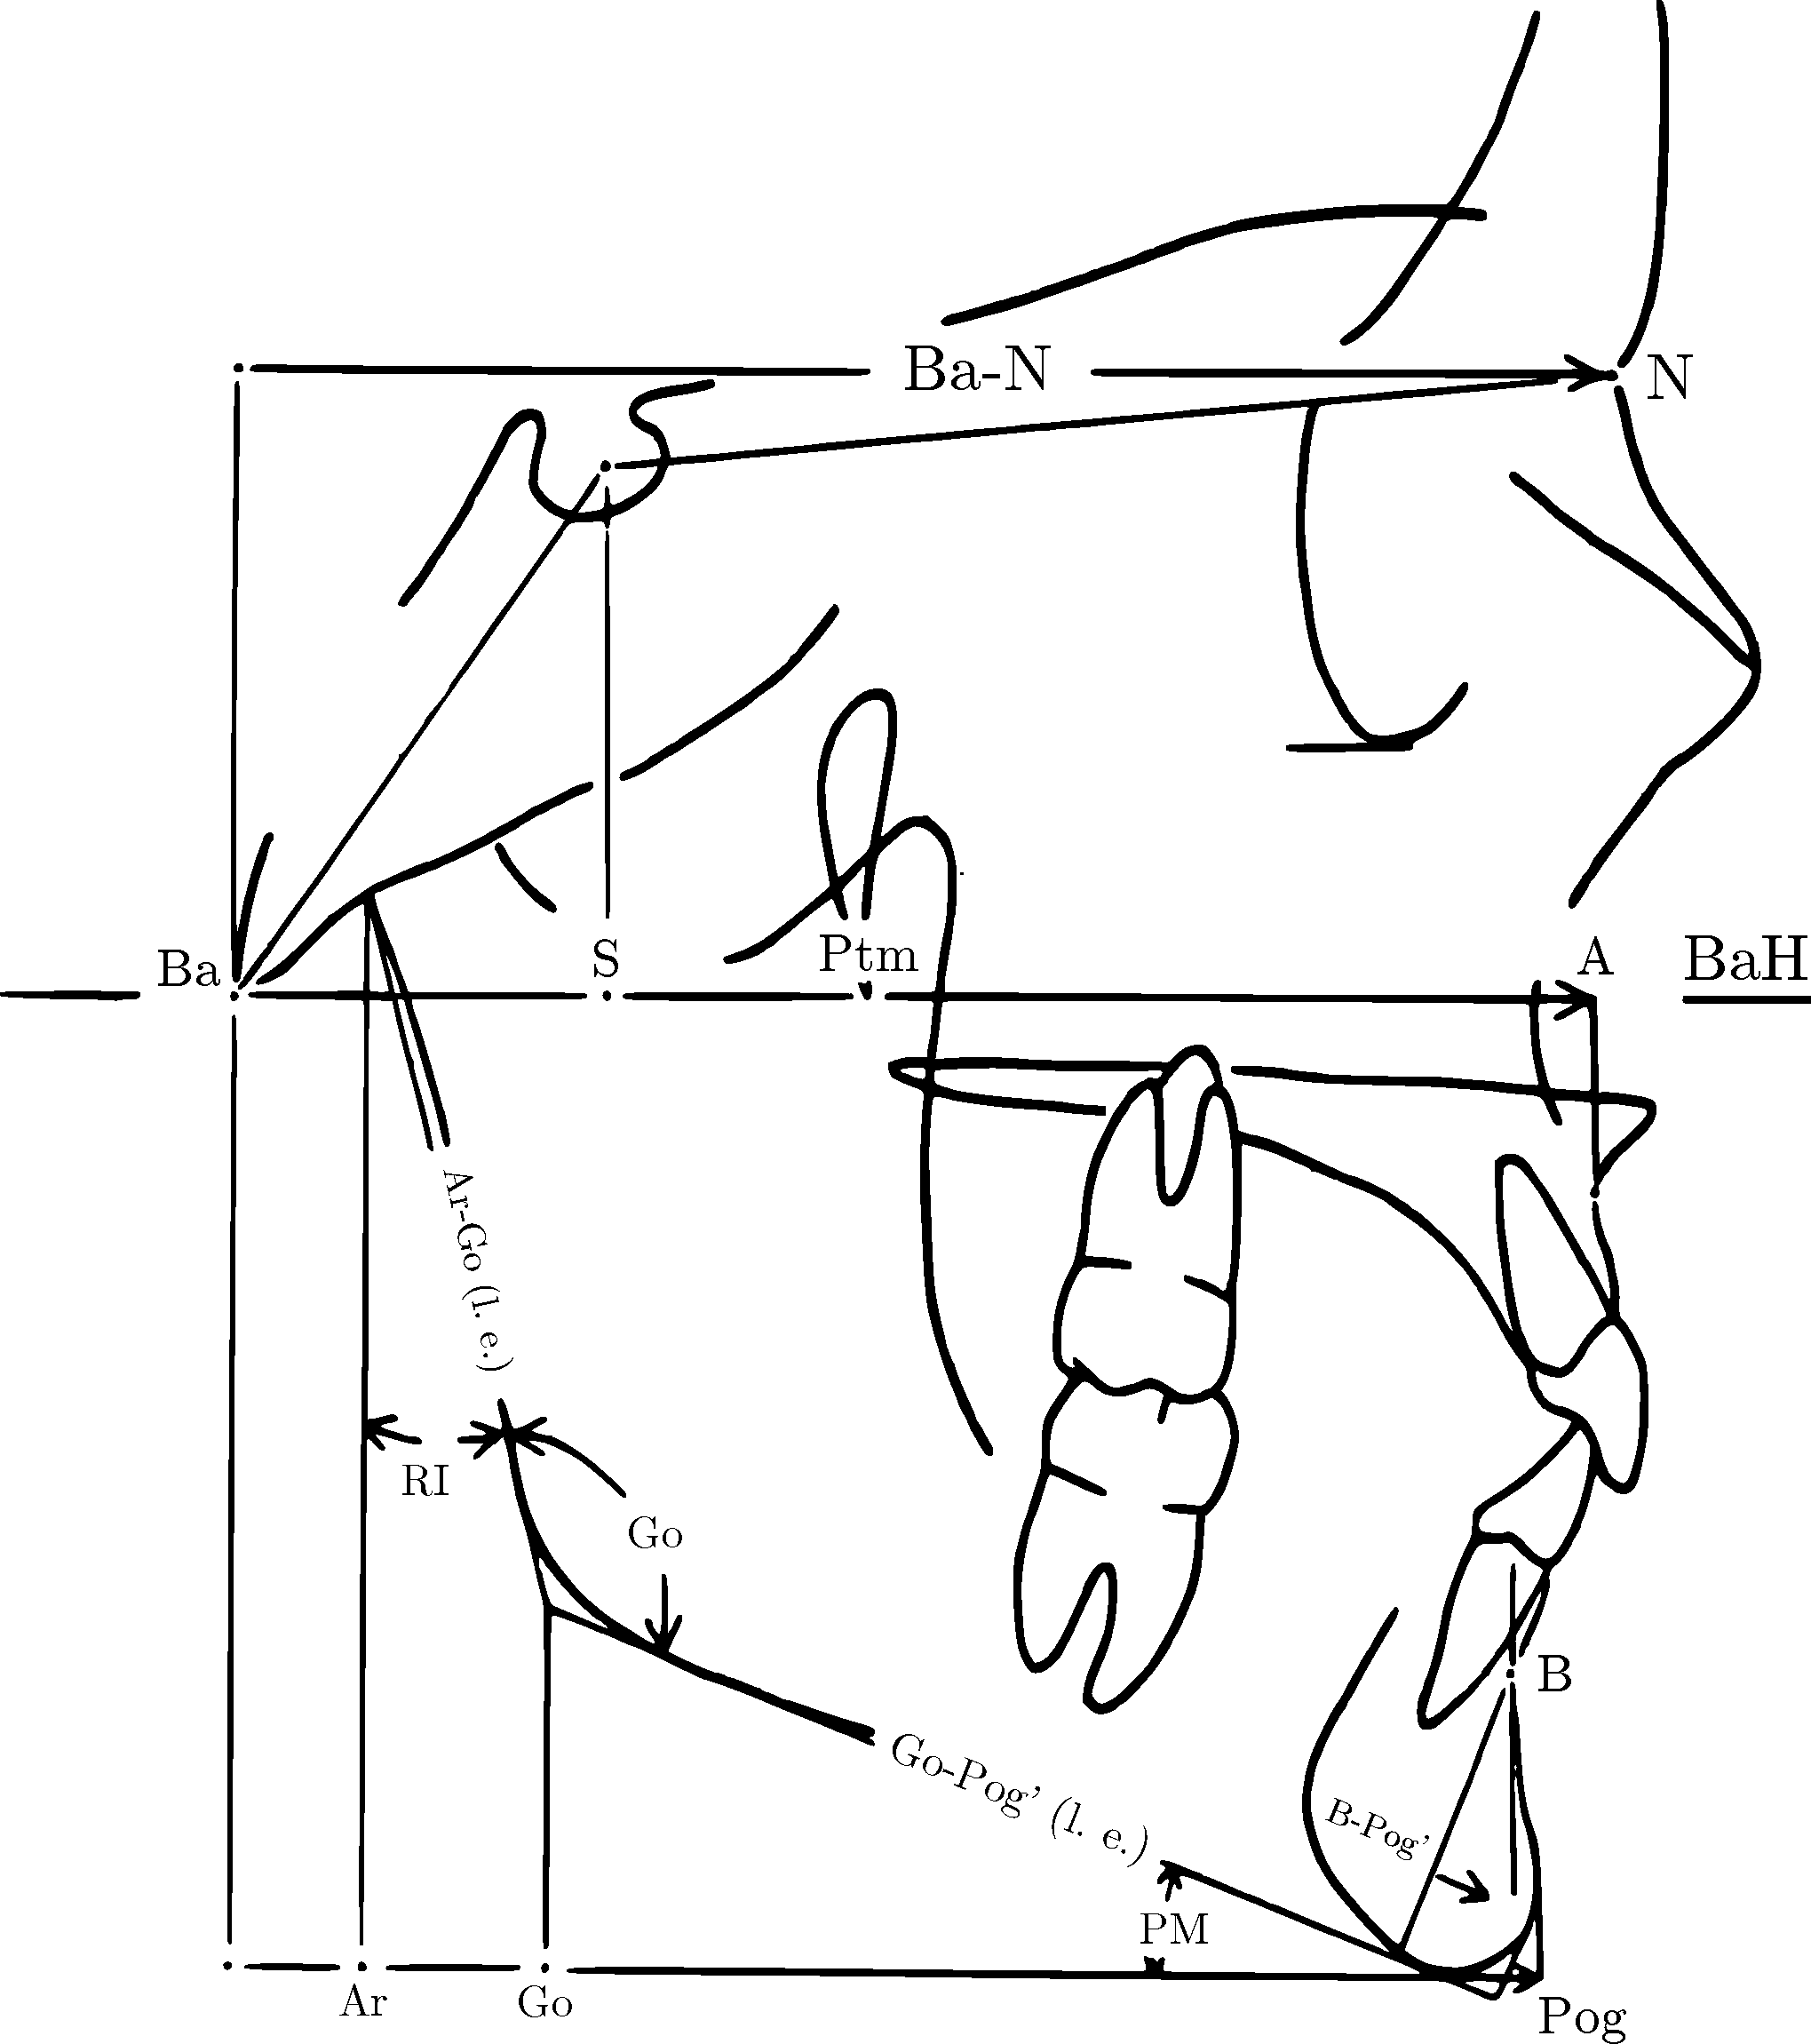
\includegraphics[width=.6\columnwidth]{./images/coben_profondita_facciale.pdf}
\caption{Analisi della profondità facciale secondo Coben}
\label{fig:coben_profondita_facciale}
\end{figure}

\paragraph{Profondità facciale inferiore} viene valutata in maniera simile: la profondità effettiva totale è misurata come \piano{Ba}{Pog}, sempre parallelamente a \punto{BaH}. Anche questo segmento può essere suddiviso in più tratti: \piano{Ba}{Ar}, che rappresenta la posizione in senso anteroposteriore della mandibola rispetto a \punto{Ba}; \piano{Ar}{Pog} che è l'effettivo contributo della mandibola alla profondità facciale inferiore . Il segmento \piano{Ba}{B} rappresenta profondità della base alveolare mandibolare relativa a \punto{Ba}, espressa come l'effettiva profondità facciale meno l'effettiva profondità del mento ($\piano{Ba}{Pog} - \piano{B}{Pog}$).

Similarmente all'analisi della base cranica, il contributo effettivo della mandibola (\piano{Ar}{Pog} -- $80,2 \pm 6,48\%$ di \piano{Ba}{N}) dipende dalle dimensioni, dalla forma e dalla posizione della mandibola stessa. In quest'analisi, questo segmento viene ulteriormente suddiviso in contributo dell'in\-cli\-na\-zio\-ne del ramo (\piano{Ar}{Go}, dove \punto{Go} è il punto costruito geometricamente, non riferito al margine osseo) e in contributo del corpo mandibolare (\piano{Go}{Pog}).

\subparagraph{Contributo del ramo} La profondità effettiva dell'inclinazione del ramo (\piano{Ar}{Go}) risulta dalla lunghezza del ramo, misurata lungo il suo margine posteriore da \punto{Ar} a \punto{Go}, e dall'inclinazione del piano del ramo, tangente al suo margine postero-inferiore, indicato con \punto{RI}$\measuredangle$. Quest'ultimo viene misurato relativo a \punto{BaV}, ed esprime il grado di deviazione del ramo da questa verticale. Un'ante-inclinazione viene, convenzionalmente, indicata con numeri positivi; il contrario con una post-inclinazione. Maggiore è il \punto{RI}$\measuredangle$, cioè più il ramo si allontana dalla verticale, maggiore è il suo contributo alla profondità facciale inferiore, e viceversa. Nel caso di un angolo \punto{RI}$\measuredangle$ negativo, una crescita del ramo causerebbe un arretramento del mento, causando una diminuzione della profondità facciale inferiore effettiva.

\subparagraph{Contributo del corpo} \piano{Go}{Pog} varia con la lunghezza assoluta del corpo mandibolare \piano{Go}{Pog'}, dove \punto{Pog'} è la sproiezione perpendicolare al piano mandibolare di \punto{Pog'}, e con l'angolo del piano mandibolare \punto{PM}$\measuredangle$. Quest'ultimo è l'angolo formato dal piano mandibolare e \punto{BaH} (o \punto{FH}, essendo equivalenti). Più piccolo è quest'angolo, maggiormente la crescita del corpo mandibolare contribuisce alla profondità facciale inferiore.

Sul piano \piano{Go}{Pog'} è possibile misurare il segmento \piano{B'}{Pog'} (anche in questo caso, \punto{B'} è sproiettato perpendicolarmente): questo è il \emph{mento anatomico}, e indica la posizione della base alveolare mandibolare rispetto al punto più prominente della sinfisi mentoniera. La differenza tra il mento anatomico e l'effettiva profondità del mento \piano{B}{Pog} (misurato parallelamente a \punto{BaH}) varia in funzione dell'inclinazione del piano mandibolare. Con la riduzione di quest'angolo verso $0°$, \piano{B}{Pog} tende ad uguagliare \piano{B'}{Pog'}. Al contrario, con l'aumento dell'angolo del piano mandibolare, l'effettiva profondità del mento tende a 0, fino a diventare negativa quando \punto{Pog} finisce posteriormente a \punto{B}.

Similarmente all'angolo della base cranica, gli effetti dell'angolo goniaco \punto{Go}$\measuredangle$ sul contributo della mandibola alla profondità e all'altezza facciale inferiore vengono valutati insieme agli angoli \punto{PM}$\measuredangle$ e \punto{RI}$\measuredangle$, secondo la relazione:
\begin{equation}
Go\measuredangle = RI\measuredangle + PM\measuredangle + 90°
\end{equation}

\section{Altezza facciale}
\begin{table}[ht]
\centering
\caption{Valori medi dell'altezza facciale nell'analisi di Coben}
\label{tab:coben_altezza_facciale}
\begin{tabular}{lcD{,}{,}{3.3}D{,}{,}{3.3}}
\toprule
\multicolumn{1}{c}{\textbf{Segmento}} & \multicolumn{1}{c}{\textbf{Riferimento}} & \multicolumn{1}{c}{\textbf{Valore medio}} & \multicolumn{1}{c}{\textbf{Dev. Std.}} \\
\midrule
\piano{N}{Me} & \piano{Ba}{N} & 115,3 \% & 6,56 \\
\piano{Ba}{S} & \piano{N}{Me} & 34,1 \% & 2,28 \\
\piano{S}{N} & & 7,1 \% & 3,68 \\
\piano{Ba}{N} & & 41,2 \% & 3,80 \\
\piano{Ba}{Go} & & 30,9 \% & 3,27 \\
\piano{Ba}{Ar} & & -7,6 \% & 1,96 \\
\piano{Go}{Me} & & 27,9 \% & 3,35 \\
\piano{S}{Go} & & 65,0 \% & 3,79 \\
\piano{Ba}{SNP} & & -2,2 \% & 2,83 \\
\piano{Ba}{SNA} & & -4,6 \% & 4,68 \\
\piano{N}{SNA} & & 45,8 \% & 2,18 \\
\piano{SNA}{$\underline{1}$} & & 23,8 \% & 2,18 \\
\piano{Me}{$\overline{1}$} & & 33,4 \% & 1,76 \\
\piano{$\underline{1}$}{$\overline{1}$} & & -3,0 \% & 2,45 \\
\piano{SNA}{Me} & & 54,2 \% & 2,18 \\
\bottomrule
\end{tabular}
\end{table}

\begin{figure}[ht]
\centering
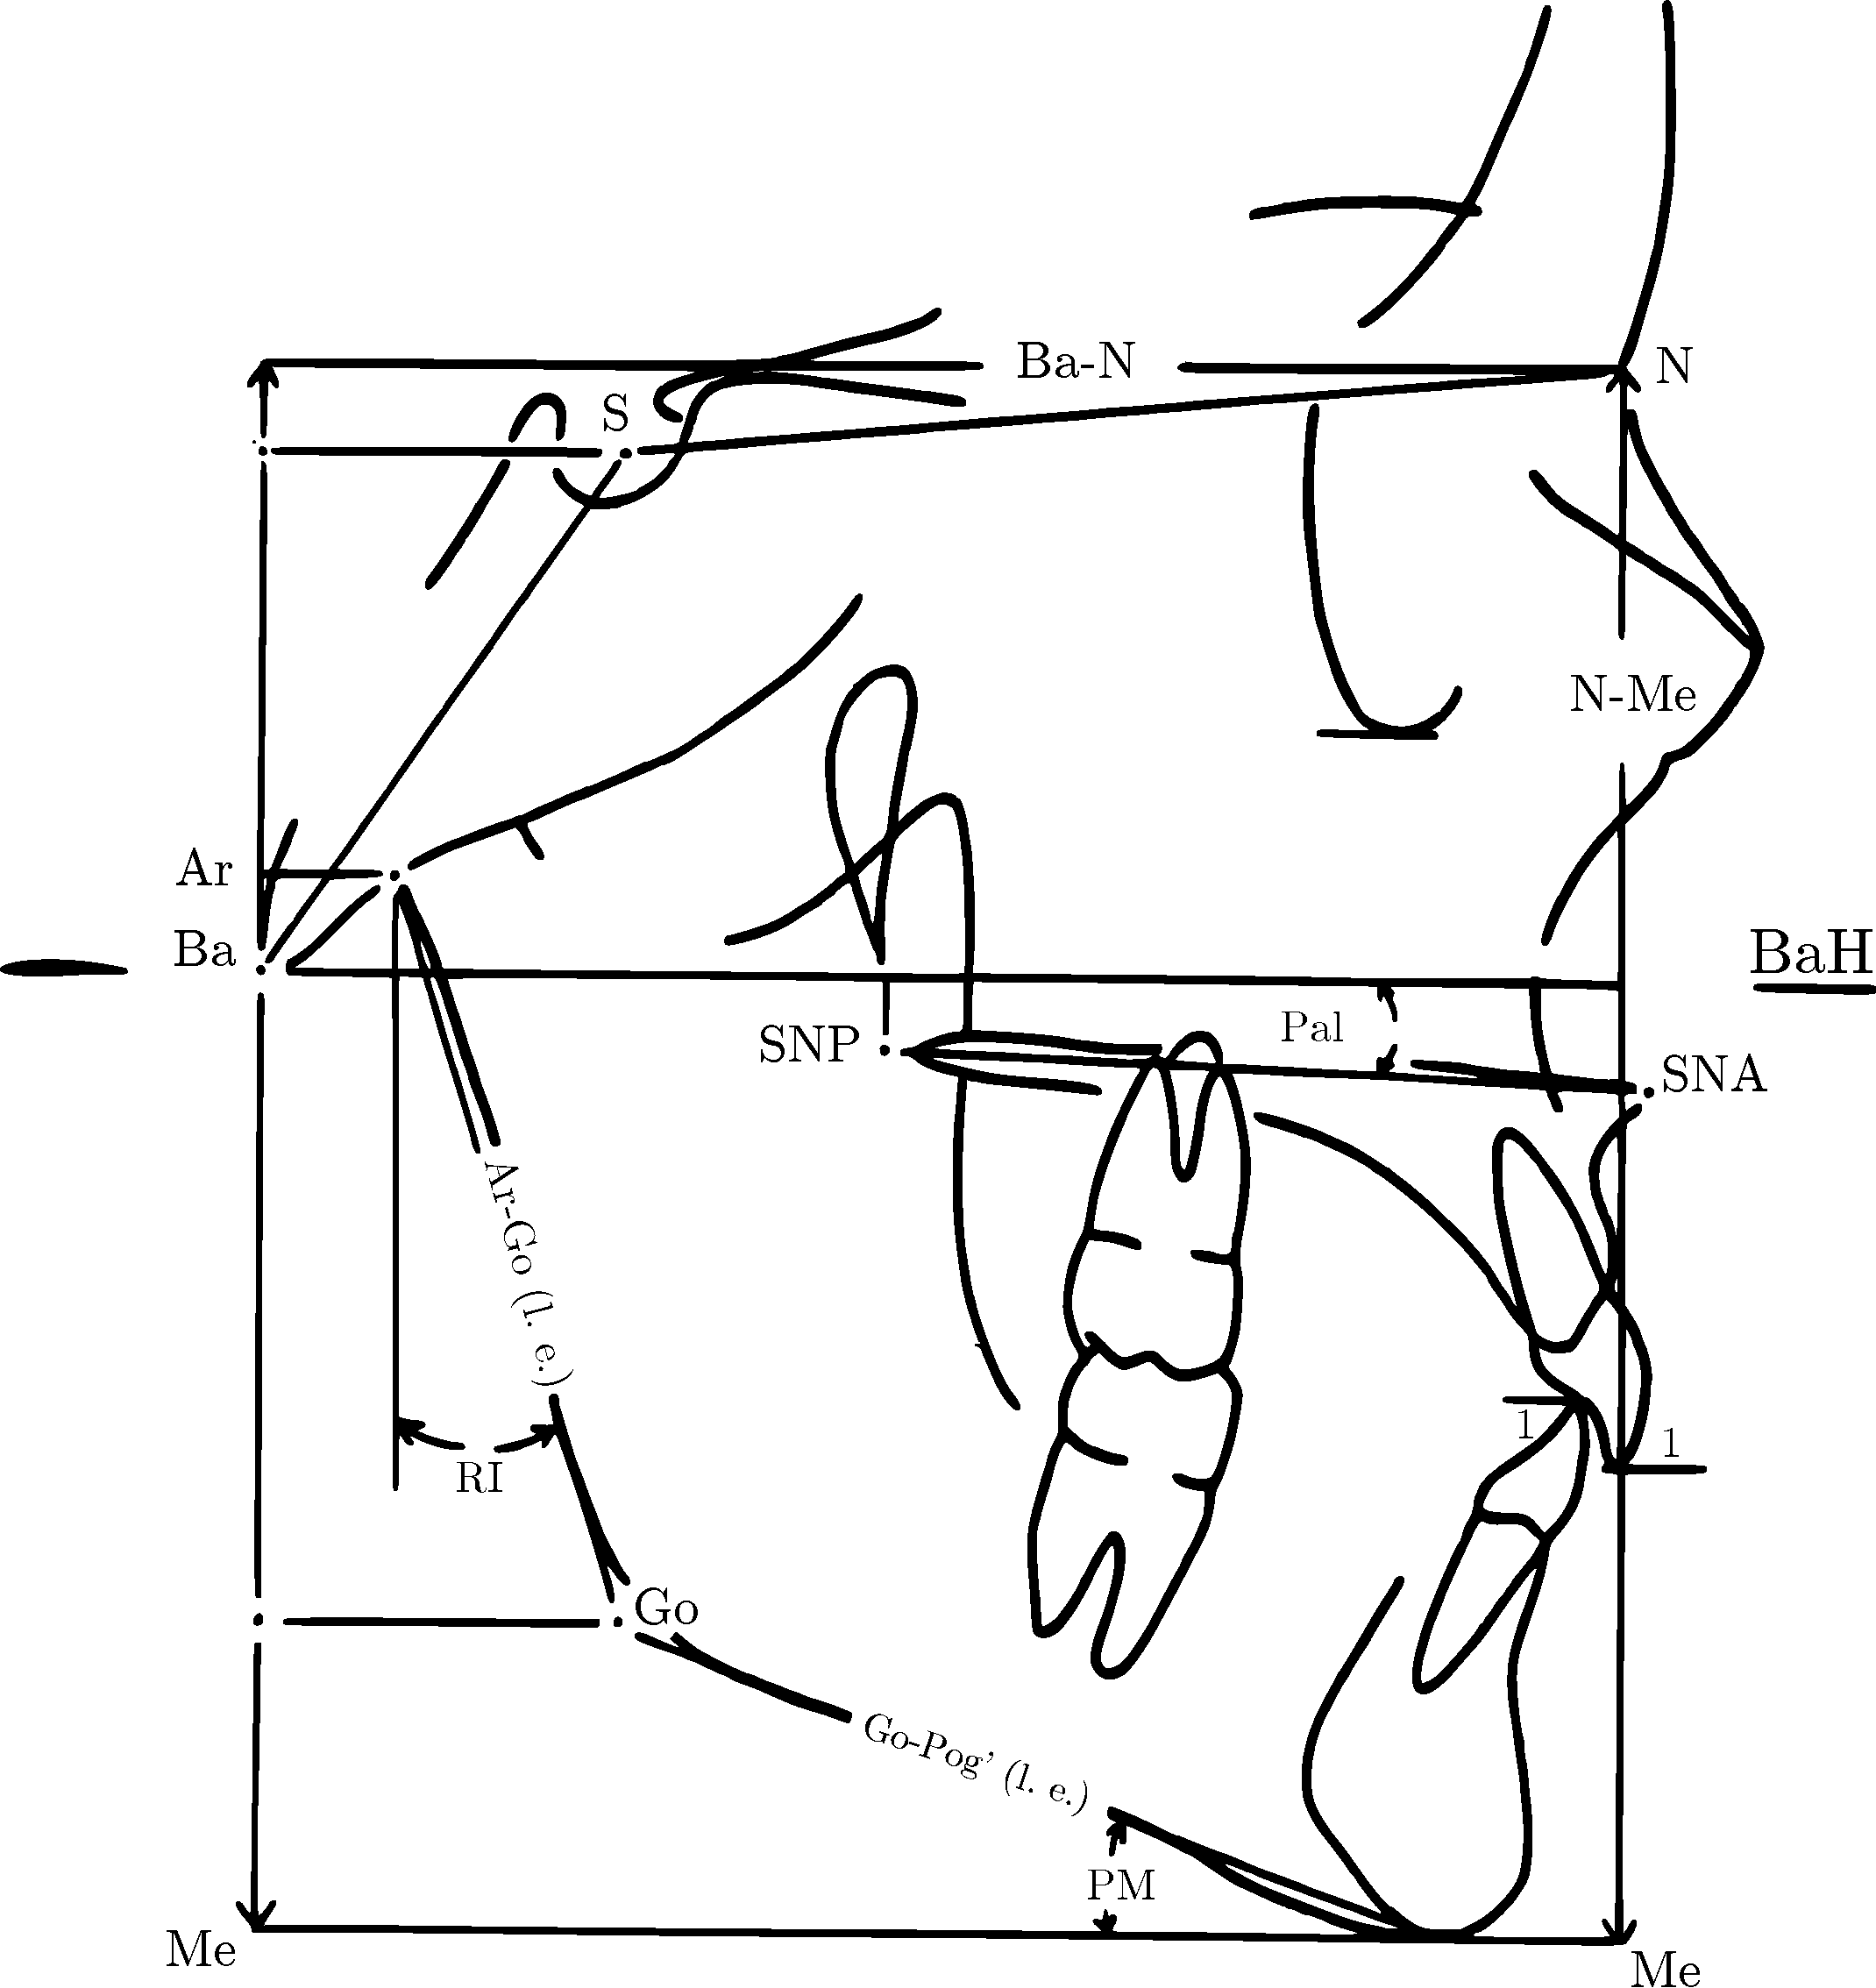
\includegraphics[width=.6\columnwidth]{./images/coben_altezza_facciale.pdf}
\caption{Analisi dell'altezza facciale secondo Coben}
\label{fig:coben_altezza_facciale}
\end{figure}

Per meglio comprendere lo sviluppo dell'altezza facciale, è necessario considerare l'altezza facciale anteriore totale \piano{N}{Me} come la risultante della divergenza del vettore di crescita della base cranica e del vettore di crescita mandibolare. Il primo porta la parte superiore della faccia in avanti e in alto, lontano dal \emph{forame magno}; il secondo spinge in basso e al davanti dello stesso. Tra i due divergenti vettori di crescita si crea uno spazio, utile per lo sviluppo della porzione superiore della faccia, per il rimodellamento del palato e l'eruzione dentaria. In questa prospettiva, il tratto \piano{N}{Me} può essere suddiviso in più componenti che rispecchino i processi di crescita: il tratto \piano{Ba}{N} che esprime la crescita della base cranica, e il tratto \piano{Ba}{Me} che esprime la crescita mandibolare.

La componente \piano{Ba}{N} risulta derivante dalla somma delle componenti verticali \piano{Ba}{S} (altezza effettiva della base cranica posteriore) e \piano{S}{N} (altezza effettiva della base cranica anteriore). Come già precedentemente enunciato, anche in questo caso le altezze effettive sono influenzate dagli angoli \punto{BaS}$\measuredangle$ e \punto{SN}$\measuredangle$, rispettivamente.

La componente \piano{Ba}{Me} è espressione dell'altezza facciale inferiore, ed è la risultante delle componenti \piano{Ba}{Go} e \piano{Go}{Me}. La prima rappresenta l'altezza facciale inferiore posteriore, ed è la risultante della componente \piano{Ar}{Go}, che rappresenta l'altezza effettiva del ramo, meno la componente supriore \piano{Ba}{Ar}. Così come nell'analisi di profondità, l'altezza effettiva del ramo \piano{Ar}{Go} varia in funzione della sua lunghezza assoluta e dell'inclinazione del ramo (\punto{RI}$\measuredangle$). Più è piccolo quest'angolo (cioè più è inclinato il ramo), più la lunghezza e la crescita del ramo contribuiscono all'altezza facciale inferiore. La componente \piano{Go}{Me} rappresenta l'altezza effettiva del corpo mandibolare, e risulta dalla lunghezza \piano{Go}{Pog'} e l'angolo \punto{PM}$\measuredangle$. Maggiore è quest'angolo, maggiore è il contributo della crescita del corpo mandibolare all'altezza facciale inferiore.

La posizione verticale del piano palatale e la sua angolazione rispetto al \punto{BaH} vengono messe in evidenza dai segmenti \piano{Ba}{SNP} e \piano{Ba}{SNA}, e dall'angolo palatale rispetto a \punto{BaH} (\punto{Pal}$\measuredangle$). Nel caso \punto{SNP} non sia visibile radiograficamente, lo si può costruire come il punto d'intersezione tra l'ordinata di \punto{Ptm} e il piano palatale. Quando \punto{SNP} o \punto{SNA} risulta essere superiore al piano \punto{BaH}, essi vengono considerati con numeri positivi, viceversa se risultano inferiori al piano di riferimento. Quando \punto{SNA} è inferiore a \punto{SNP}, il piano palatale è ruotato verso il basso, e l'angolo palatale viene considerato positivo; viceversa se \punto{SNA} è superiore a \punto{SNP}.

Nella quantificazione dell'altezza facciale anteriore, l'altezza totale \piano{N}{Me} risulta essere costituita dai tratti \piano{N}{SNA} e \piano{SNA}{Me}. Quest'ultimo è la risultante dell'altezza dentale superiore \piano{SNA}{$\underline{1}$} e l'altezza dentale inferiore \piano{Me}{$\overline{1}$}, meno l'overbite o più l'openbite \piano{$\underline{1}$}{$\overline{1}$}.

\section{Analisi dentale}
Nell'analisi della dentatura vengono considerate la posizione e inclinazione dei primi molari e degli incisivi centrali, in relazione a \punto{Ba}.

\begin{figure}
\centering
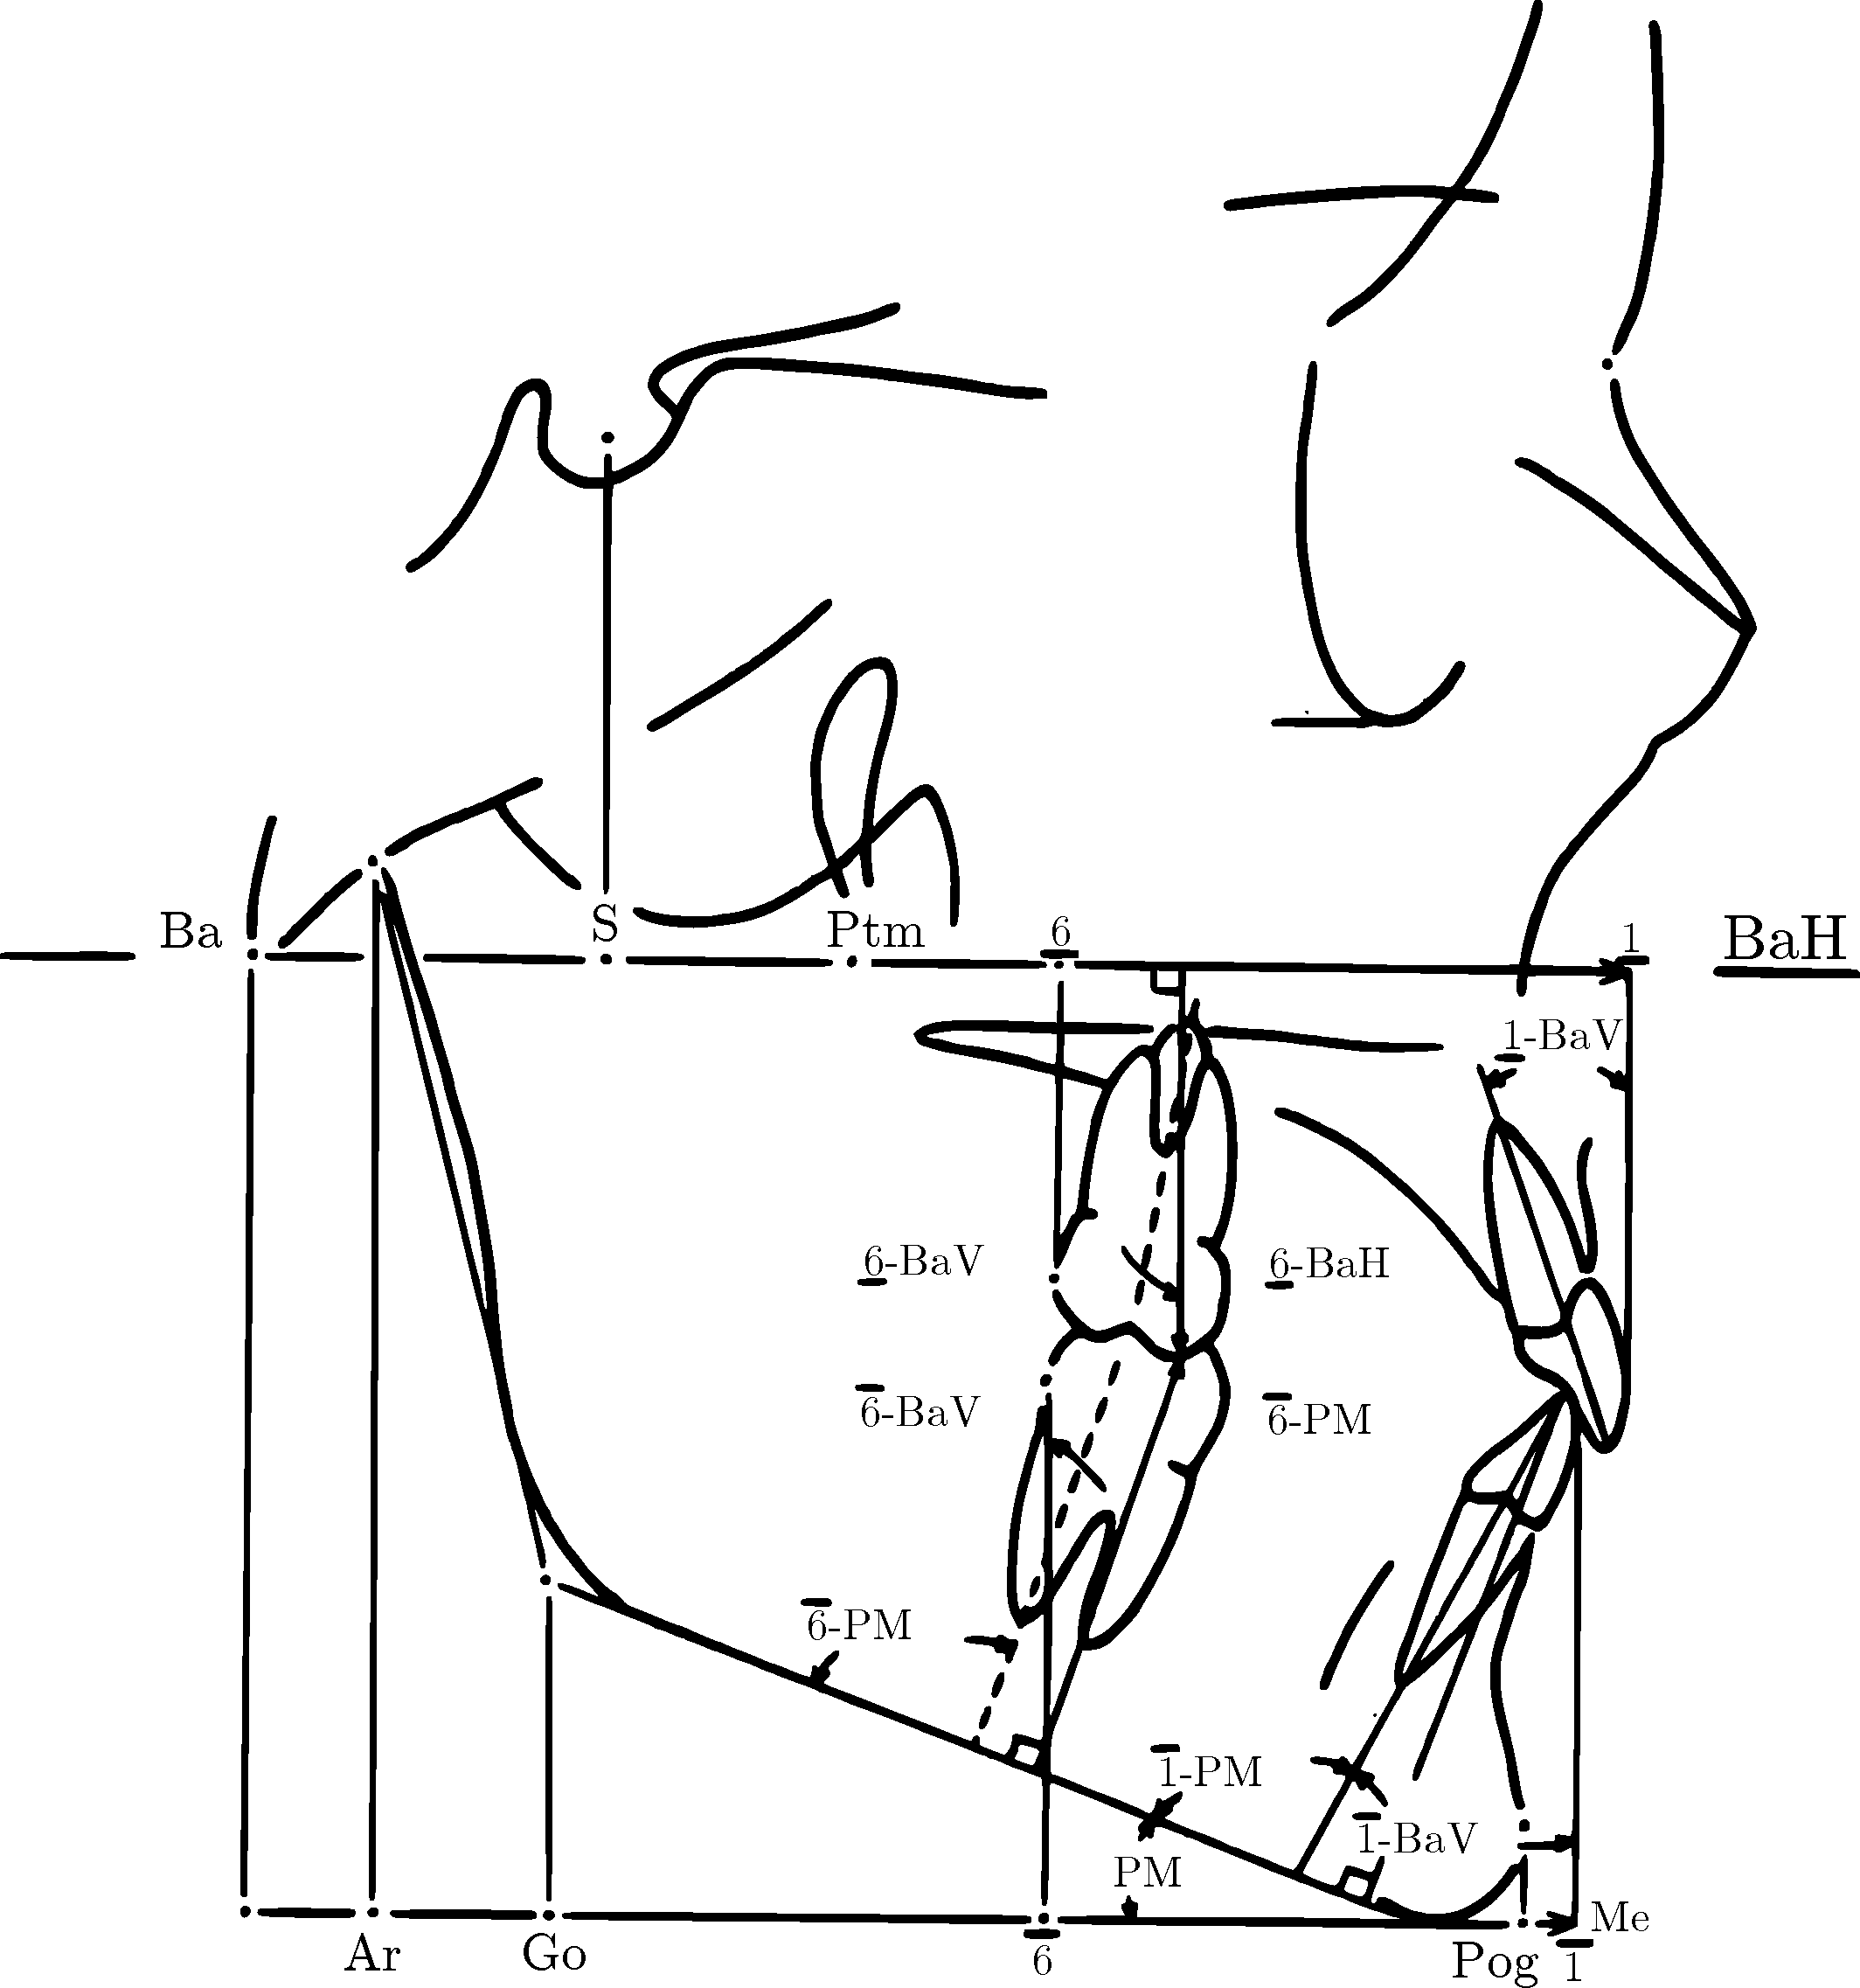
\includegraphics[width=.6\columnwidth]{./images/coben_dentale.pdf}
\caption{Analisi dentale secondo Coben}
\label{fig:coben_dentale}
\end{figure}

\subsection*{Primi molari}
La profondità del primo molare permanente mascellare \piano{Ba}{$\underline{6}$} risulta essere la somma dela profondità della base cranica posteriore \piano{Ba}{S}, più la dimensione \piano{S}{Ptm}, più la posizione del molare relativa a \punto{Ptm} \piano{Ptm}{$\underline{6}$}. Similarmente viene valutato il primo molare permanente inferiore: la distanza \piano{Ba}{$\overline{6}$} risulta essere la somma di \piano{Ba}{Ar} più l'effettiva profondità del ramo \piano{Ar}{Go}, più la posizione del molare relativa a \punto{Go} \piano{Go}{$\overline{6}$}.

Il molare inferiore viene traslato in avanti dalla crescita mandibolare, in maniera uguale all'aumento della profondità inferiore facciale \piano{Ba}{Pog}: perciò ogni differenza tra le due misurazioni viene interpretato come un movimento mesiale o distale nell'ambito del corpo stesso, ed è uguale alla lunghezza \piano{$\overline{6}$}{Pog}. Questo è vero per tutte le fasi di crescita, con l'eccezione degli stadi tardivi quando è possibile un rimodellamento della sinfisi.

Verticalmente, la posizione del sesto superiore viene misurata perpendicolarmente a \punto{BaH} tramite la cuspide mesio-vestibolare (\piano{$\underline{6}$}{BaH}), e l'inclinazione viene riferita a \punto{BaV} (\punto{$\underline{6}$BaV}$\measuredangle$). Il primo molare inferiore viene misurato similarmente al superiore, in maniera perpendicolare al piano mandibolare (\piano{$\overline{6}$}{PM}$\perp$), e l'inclinazione viene riferita anch'essa a \punto{BaV} (\punto{$\overline{6}$BaV}$\measuredangle$). L'inclinazione del sesto inferiore rappresenta l'effetto combinato dell'angolo del piano mandibolare \punto{PM}$\measuredangle$ più l'inclinazione del molare relativo al piano mandibolare \punto{$\overline{6}$PM}$\measuredangle$. Questa relazione è espressa dall'equazione:
\begin{equation}
\overline{6}BaV\measuredangle = PM\measuredangle + \overline{6}PM\measuredangle - 90°
\end{equation}

\subsection*{Incisivi}
Similarmente ai molari, la posizione degli incisivi viene riferita a \punto{Ba}. La posizione orizzontale dell'incisivo superiore viene misurata lungo \punto{BaH} fino alla superficie più labiale dell'incisivo (\piano{Ba}{$\underline{1}$}, la posizione verticale viene misurata su \punto{BaV} come la distanza tra \punto{BaH} e la proiezione del margine incisale (\piano{$\underline{1}$}{BaH}), l'inclinazione viene riferita a \punto{BaV} (\punto{$\underline{1}$BaV}$\measuredangle$).

Similarmente si valuta l'incisivo inferiore, con la differenza che la posizione verticale viene inizialmente riferita alla perpendicolare al piano mandibolare (\piano{$\overline{1}$}{PM}$\perp$), quindi da \punto{Me} lungo \punto{BaV} fino alla proiezione del margine incisale (\piano{$\overline{1}$}{Me}) come altezza effettiva. { \huge FIXME }. L'inclinazione viene misurata su \punto{BaV}, e risulta essere l'effetto combinato dell'angolo del piano mandibolare \punto{PM}$\measuredangle$ più l'inclinazione dell'incisivo relativo al piano mandibolare \punto{$\overline{1}$PM}$\measuredangle$. Questa relazione è espressa dall'equazione:
\begin{equation}
\overline{1}BaV\measuredangle = PM\measuredangle + \overline{1}PM\measuredangle - 90°
\end{equation}

\section{Profilo}

\begin{figure}
\centering
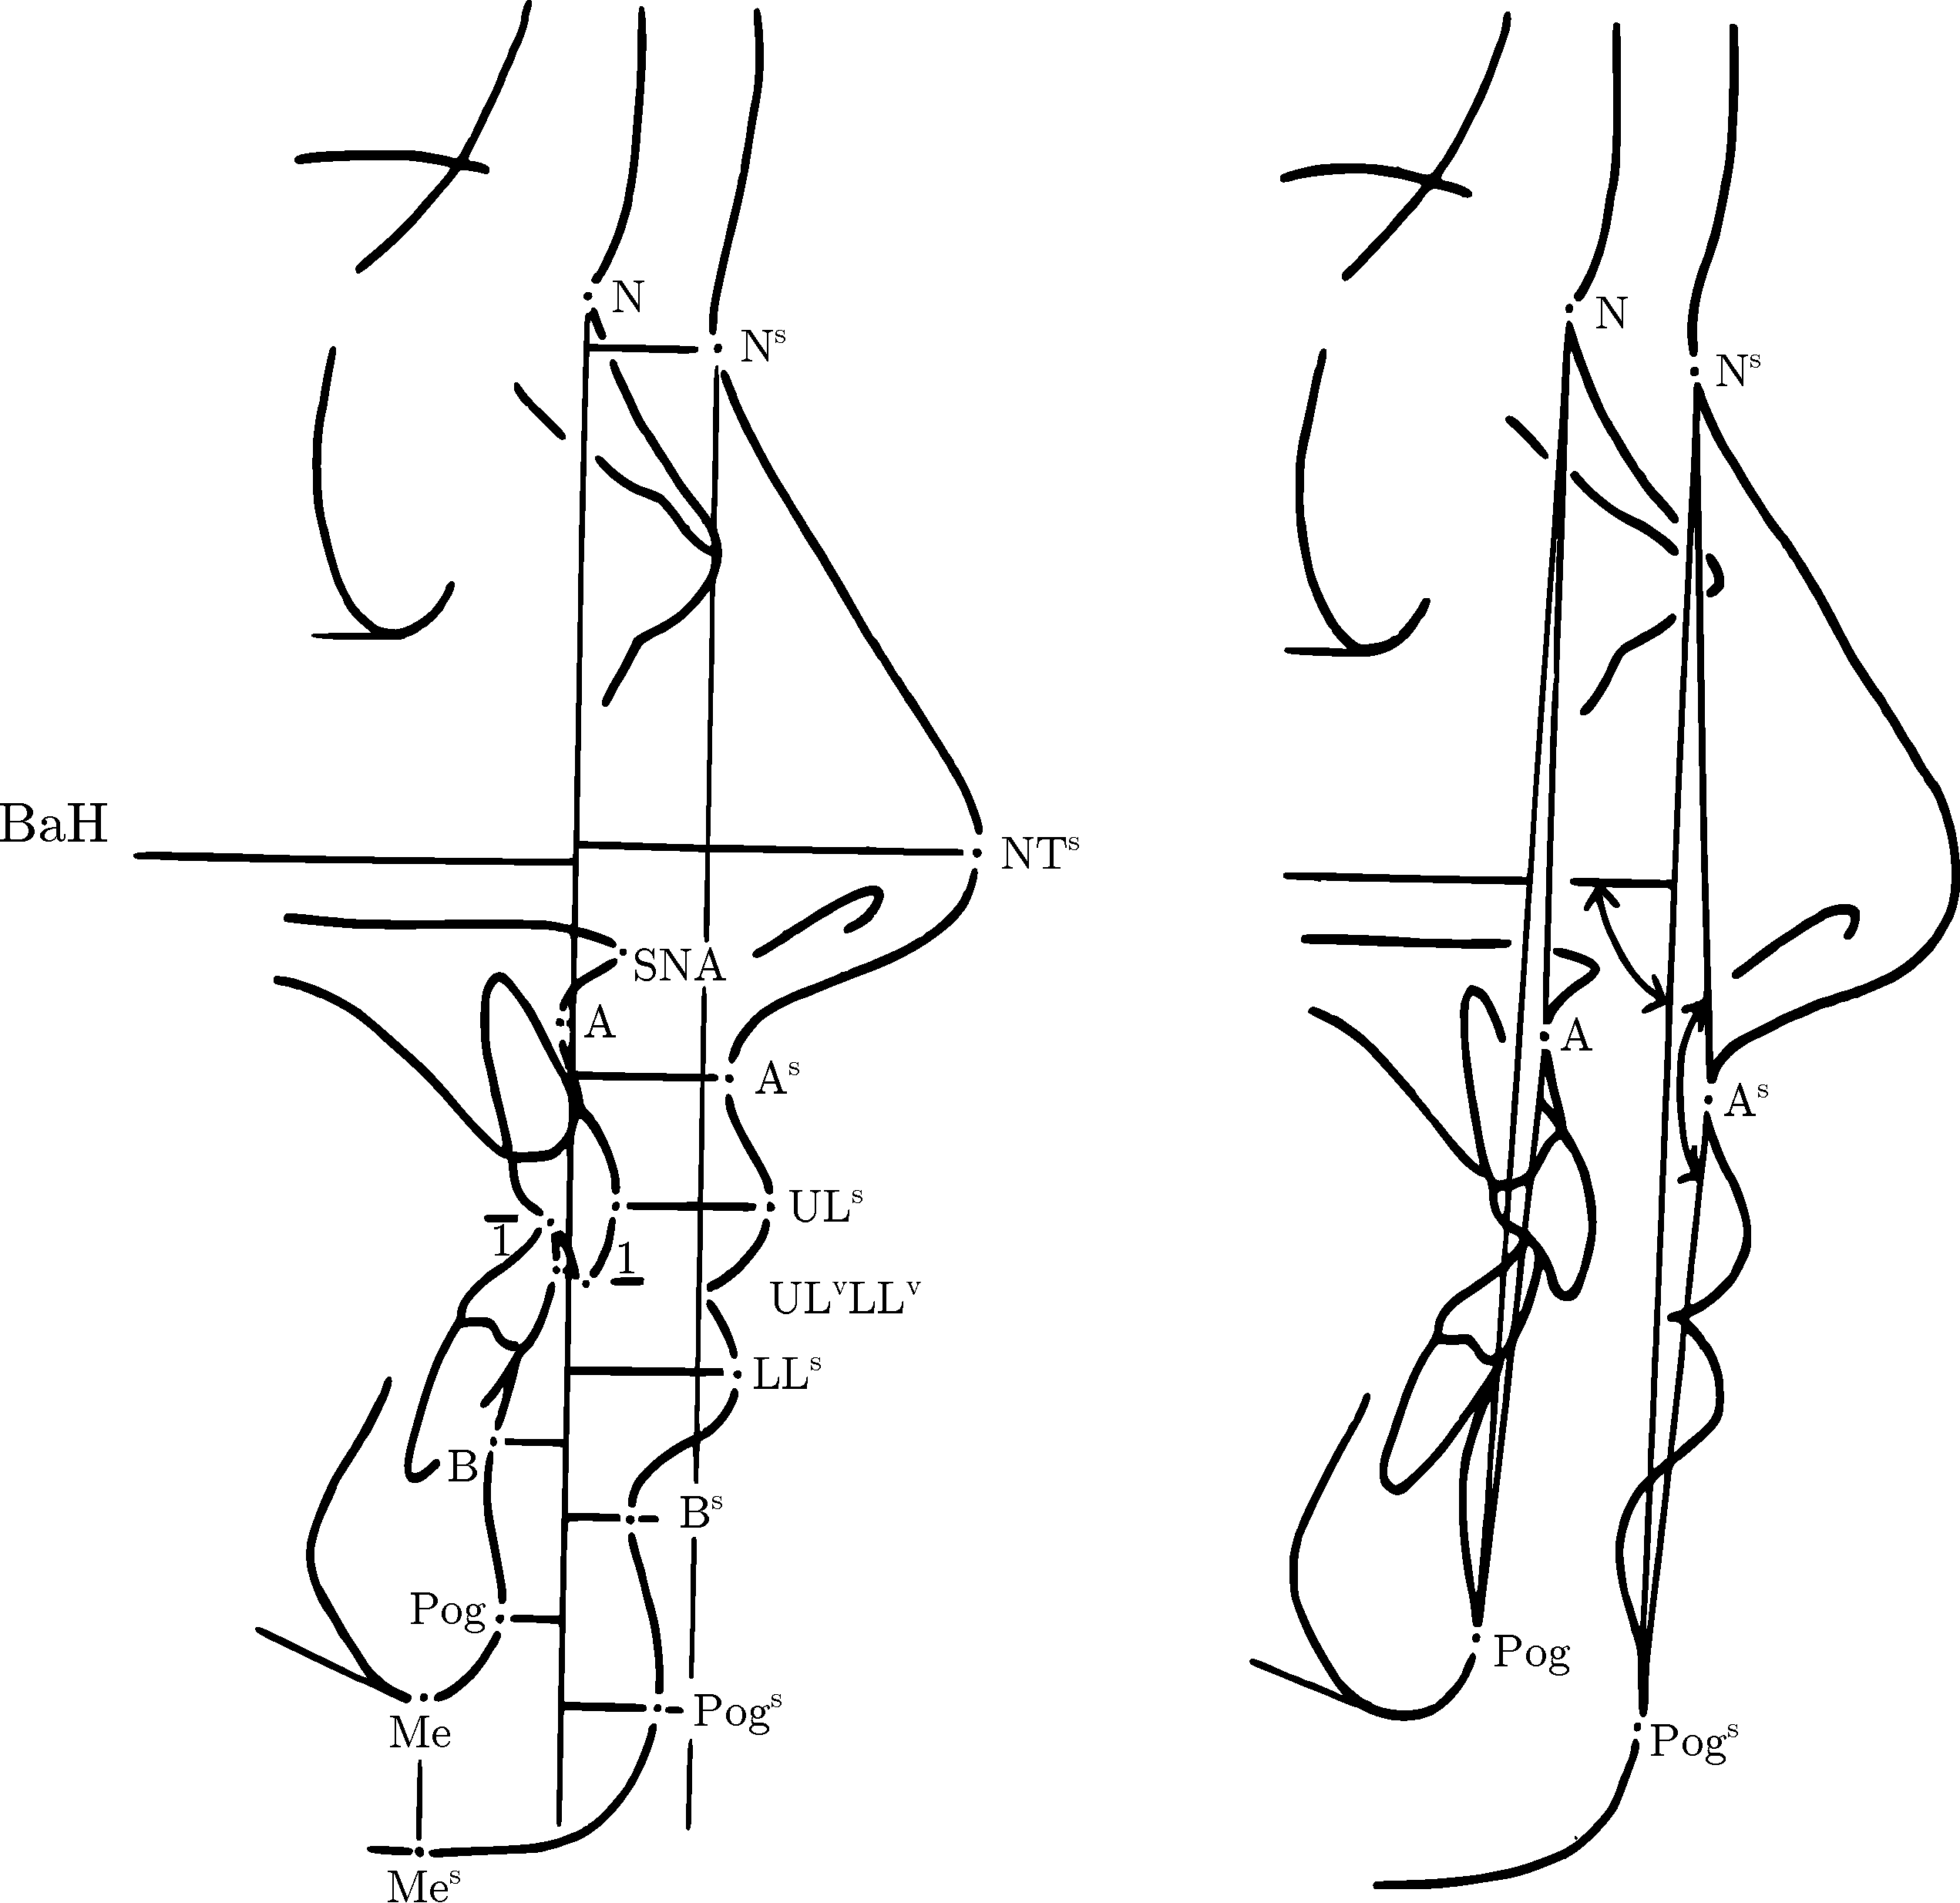
\includegraphics[width=.6\columnwidth]{./images/coben_profilo.pdf}
\caption{Analisi del profilo secondo Coben}
\label{fig:coben_profilo}
\end{figure}

L'analisi del profilo dei tessuti molli rende possibile evidenziare la correlazione tra la crescita scheletrica, lo spessore dei tessuti molli e i conseguenti cambiamenti nel profilo. L'analisi paragona il profilo scheletrico e cutaneo, e quantifica le differenze utilizzando punti di repere scheletrici e cutanei paragonabili.
\subsection*{Tipologia di profilo}
Il tipo facciale del profilo scheletrico e dei tessuti molli  sono paragonati misurando l'angolo facciale scheletrico di Downs e l'angolo della convessità facciale di Downs, e i corrispettivi sui tessuti molli.
\subsection*{Profondità}
Inizialmente vengono misurate le profondità sul piano scheletrico, riferite su \punto{BaV} passante per \punto{N}; come positive se anteriori e negative se posteriori, e in particolare \piano{N}{SNA}, \piano{N}{A}, \piano{N}{$\underline{1}$}, \piano{N}{$\overline{1}$}, \piano{N}{B} e \piano{N}{Pog}. Quindi vengono effettuate le stesse misure sul piano cutaneo, usando i punti omologhi. Successivamente vengono valutati gli spessori dei tessuti molli, valutando la differenza orizzontale tra punti comparabili: \piano{N}{N$^s$}, \piano{SNA}{punta del naso$^s$}, \piano{A}{A$^s$}, \piano{$\underline{1}$}{UL$^s$}, \piano{$\overline{1}$}{LL$^s$}, \piano{B}{B$^s$} e \piano{Pog}{Pog$^s$}.
\subsection*{Altezza}
Vengono inizialmente misurate le relazioni scheletriche, cioè \piano{N}{Me}, \piano{N}{SNA}, \piano{SNA}{$\underline{1}$}, \piano{Me}{$\underline{1}$}, \piano{$\underline{1}$}{$\overline{1}$}, \piano{SNA}{Me}. Successivamente, vengono misurate le differenze verticali tra punti di repere comparabili: \piano{N$^s$}{Me$^s$}, \piano{N$^s$}{punta del naso$^s$}, \piano{punta del naso$^s$}{UL$^v$}, \piano{Me$^s$}{LL$^v$}, \piano{UL$^v$}{LL$^v$}, \piano{punta del naso$^s$}{Me$^s$}. Quindi vengono misurate le differenze tra punti scheletrici e cutanei omologhi: \piano{N}{N$^s$}, \piano{SNA}{punta del naso$^s$}, \piano{SNA}{UL$^v$}, \piano{$\underline{1}$}{UL$^v$}, \piano{$\overline{1}$}{LL$^v$}, \piano{Me}{Me$^s$}, usando numeri positivi quando il punto cutaneo risulta superiore al punto scheletrico, e viceversa. Dopodiché è necessario misurare i punti rispettivamente a \punto{BaH}: \punto{N}, \punto{punta del naso$^s$}, \punto{SNA}, \punto{$\underline{1}$}, \punto{UL$^v$}, \punto{$\overline{1}$}, \punto{LL$^v$}, \punto{Me}, usando numeri positivi se superiori a \punto{BaH}, e viceversa.

% \subsubsection{Mascellare superiore}
% \begin{description}
% \item[\piano{Ba}{A}/\piano{Ba}{Na}] profondità del mascellare superiore, valore medio $97,7 \pm 1,8$\%.
% \item[\piano{S}{SNP}/\piano{Ba}{Na}] localizzazione antero-posteriore del mascellare superiore, valore medio $20,2 \pm 1,2$\%.
% \item[\piano{SNP}{A}/\piano{Ba}{Na}] dimensione sagittale del mascellare superiore, valore medio $52,1 \pm 1,8$\%.
% \end{description}
% 
% \subsubsection{Mandibola}
% \begin{description}
% \item[\piano{Ba}{Po}/\piano{Ba}{Na}] profondità della mandibola, valore medio $90,1 \pm 6,38$\%.
% \item[\piano{Ba}{Ar}/\piano{Ba}{Na}] localizzazione antero-posteriore della mandibola, valore medio $8,8 \pm 1,63$\%.
% \item[\piano{Ar}{Go}/\piano{Ba}{Na}] inclinazione posteriore del ramo, valore medio $7,8 \pm 1,77$\%.
% \item[\piano{Go}{Po}/\piano{Ba}{Na}] profondità del corpo della mandibola, valore medio $79,1 \pm 4,2$\%.
% \end{description}
% 
% \subsection{Analisi dell'equilibrio verticale}
% Si distinguono un livello anteriore ed un livello posteriore. Per quanto riguarda il primo, si considerano:
% 
% \begin{description}
% \item[\piano{Na}{Me}] è, come il \piano{Ba}{Na}, un valore assoluto individuale, a cui si rapportano tutte le misure individuali. Rappresenta l'altezza anteriore della faccia, ed ha un valore medio di $123,9 \pm 4,85$mm.
% \item[\piano{Na}{SNA}/\piano{Na}{Me}] è l'altezza del mascellare, ha un valore medio di $46 \pm 2,18$\%.
% \item[\piano{SNA}{Me}/\piano{Na}{Me}] è l'altezza inferiore della faccia, ha un valore medio di $54 \pm 2,18$\%.
% \item[\piano{SNA}{Is}/\piano{Na}{Me}] è l'altezza del processo alveolare del mascellare superiore, ha un valore medio di $23,2 \pm 1,58$\%.
% \item[\piano{Ii}{Me}/\piano{Na}{Me}] è l'altezza del processo alveolare e della sinfisi mentoniera a livello mandibolare, ha un valore medio di $34,1 \pm 1,68$\%.
% \end{description}
% 
% Per quanto riguarda il livello posteriore, si considerano:
% 
% \begin{description}
% \item[\piano{S}{Go}/\piano{Na}{Me}] rappresenta l'altezza totale posteriore della faccia, rapportata con l'altezza totale anteriore. Ha un valore medio di $68,8 \pm 2,4$\%.
% \item[\piano{S}{Ar}/\piano{Na}{Me}] rappresenta la posizione del condilo rispetto alla sella su un piano verticale, ha un valore medio di $26,5 \pm 1,84$\%.
% \item[\piano{Ar}{Go}/\piano{Na}{Me}] rappresenta l'altezza della branca ascendente, ha un valore medio di $42,3 \pm 2,41$\%.
% \end{description}
